\documentclass[a4paper,11pt, oneside]{article}

\usepackage[utf8] { inputenc }
\usepackage[T1] { fontenc } 
\usepackage[english]{babel}
\usepackage{titlesec, blindtext, color}
\definecolor{gray75}{gray}{0.75}
\newcommand{\hsp}{\hspace{20pt}}

\usepackage{amsmath}
\usepackage{amsthm}
\usepackage{amssymb}
\usepackage[titletoc]{appendix}
\usepackage{array}
\usepackage{booktabs}
\usepackage{float}
\usepackage{braket}
\usepackage{fullpage}
\usepackage{graphicx}
\usepackage{hyperref}
\usepackage{titlepic}
\usepackage [round,authoryear] {natbib}
\usepackage{ifthen}
\newtheorem{axiom}{Axiom}
\newtheorem{theorem}{Theorem}
% Set version number
\newcommand{\mydocumentversion}{0.0.2}
\usepackage{algorithm}
\usepackage{algpseudocode}
\usepackage{amsmath}


% Do not show subsections in table of contents
\setcounter{tocdepth}{1}

% Python code setup
\usepackage{pythonhighlight}

\DeclareMathOperator*{\argmax}{argmax}
\DeclareMathOperator*{\argmin}{argmin}

\theoremstyle{definition}
\newtheorem{exinn}{Example}
\newenvironment{example}
{\clubpenalty=10000
	\begin{exinn}%
		\mbox{}%
		{\color{black}\leaders\hrule height .8ex depth \dimexpr-.8ex+0.8pt\relax\hfill}%
		\mbox{}\linebreak\ignorespaces}
	{\par\kern2ex\hrule\end{exinn}}


\begin{document}
	
	
	\begin{titlepage}
		\title{\small{Competence Development}\\
			\huge{Bayesian Decision Theory Asymmetric Cost}
		}
		\author{Jonas Petersen \\ Ander Runge Walther }
		\date{} % No date on the title page
		\maketitle
		\thispagestyle{empty}
	\end{titlepage}
	
	\newpage
	\tableofcontents
	\addtocontents{toc}{\protect\thispagestyle{plain}}

	\thispagestyle{plain}
	
	
	\section{Introduction}
	This note considers how quantile regression can be derived, from a particular cost function, as the optimal decision rule using Bayesian decision theory. Consider a regression scenario where $s$ denote the true value and $U(x,D)$ the estimate based on input $x$ and data $D$. A linear asymmetric cost function can be written viz
	\begin{equation}
		C(U(x,D), s) = \alpha\cdot \text{swish}(U(x,D)-s,\beta)+(1-\alpha)\cdot\text{swish}(s-U(x,D),\beta)
		\label{eq:cost}
	\end{equation}
	where
	\begin{equation}
		\text{swish}(z,\beta) = \frac{z}{1+e^{-z\beta}}
	\end{equation}
	and $z\equiv U(x,D)-s$ for brevity. For $\beta\gg 1 $ equation \eqref{eq:cost} approximate two linear segments around Origin as shown in figure \ref{fig:1}.
	\begin{figure}[H]
		\centering
		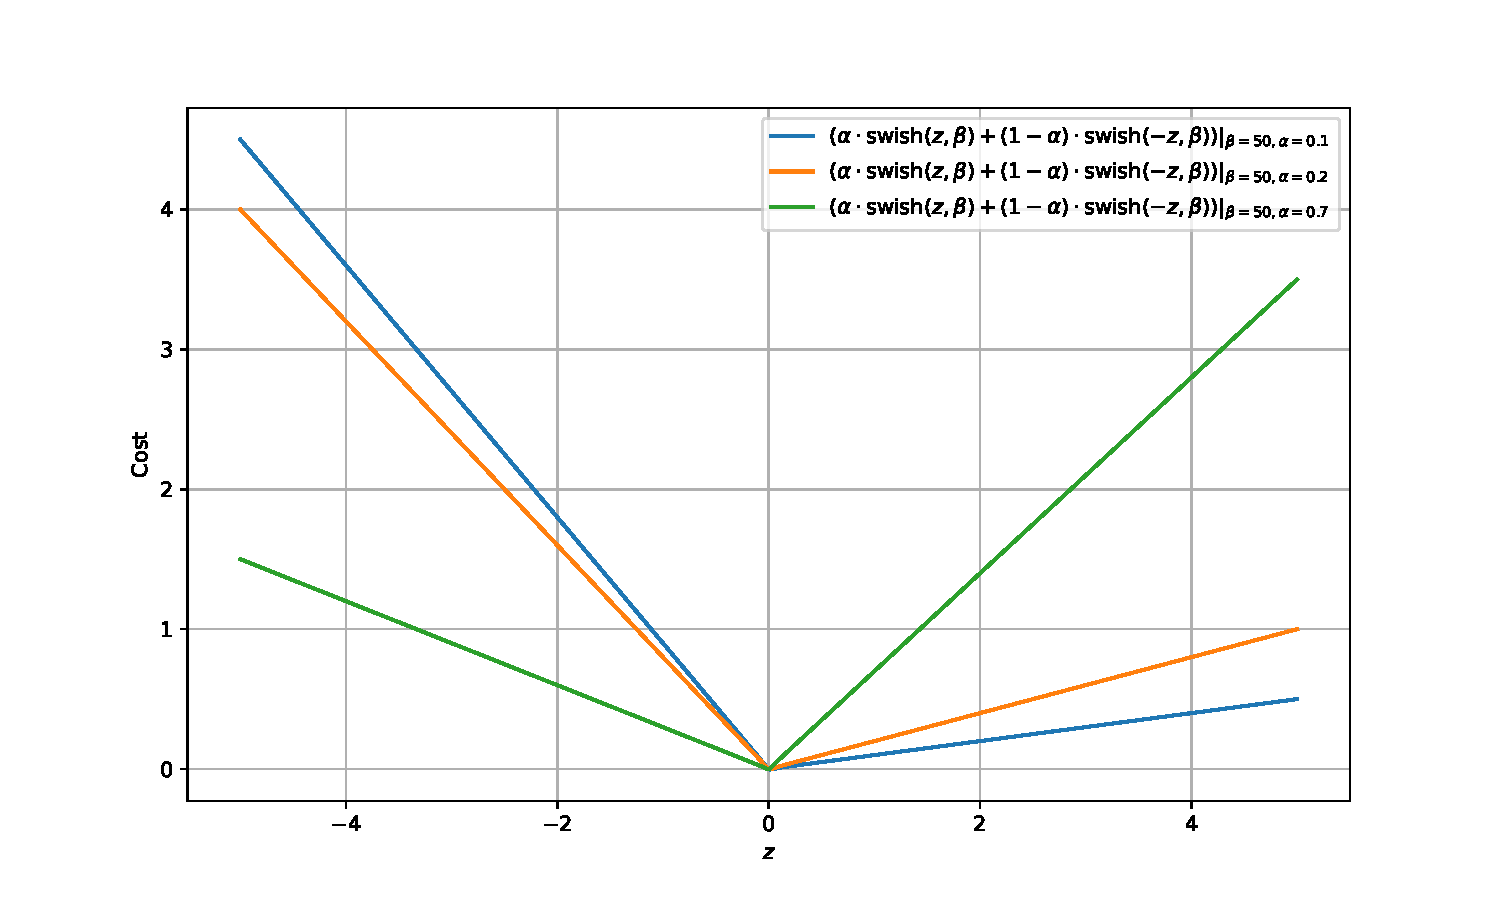
\includegraphics[width = 1\textwidth]{figures/cost_plot.pdf}
		\caption{Illustration of equation \eqref{eq:cost} with different parameter values $\alpha,\beta$.}
		\label{fig:1}
	\end{figure}
	Taking $\alpha \ll 1$, then $z<0$ will be penalized relatively more than $z>0$. $z<0$ corresponds to underestimation, so this is penalized greater relative to overestimation. Now
	\begin{equation}
		\begin{split}
			\mathbb{E}[C|x,D,I] & =\int ds p(s|x,D,I) \bigg(\alpha\cdot \text{swish}(U(x,D)-s,\beta)+(1-\alpha)\cdot\text{swish}(s-U(x,D),\beta)\bigg)
		\end{split}
		\label{eq:1}
	\end{equation}
	where $I$ denote the background information~\citep{Sivia2006}. The optimal decision rule $U^*(x,D)$ can be found from the derivative
	\begin{equation}
		\begin{split}
			\frac{dC}{dU} & = \frac{dC}{dz}\frac{dz}{dU}\\
			& = \bigg(\frac{\alpha}{1+e^{-\beta z}}-\frac{1-\alpha}{1+e^{\beta z}}+\frac{\alpha\beta e^{-\beta z}z}{(1+e^{-\beta z})^2}+\frac{(1-\alpha)\beta e^{\beta z}z}{(1+e^{\beta z})^2}\bigg)\frac{dz}{dU}\\
			&= \frac{\beta z e^{\beta z}-e^{\beta z}-1}{(1+e^{\beta z})^2}+\alpha+\mathcal{O}(\alpha^2)\\
			&\approx  \alpha -\frac{1}{(1+e^{\beta z})^2}
		\end{split}
		\label{eq:2}
	\end{equation}
	where it has been used that $\alpha\ll 1$. Combining equations \eqref{eq:1} and \eqref{eq:2} alongside imposing the derivative vanish for the optimal decision rule
	\begin{equation}
		\begin{split}
			\frac{d\mathbb{E}[C|x,D,I ]}{dU}\bigg|_{U=U^*} &\approx \int ds p(s|x,D,I) \bigg(\alpha -\frac{1}{(1+e^{\beta z})^2}\bigg)\\
			& = \alpha -\int ds p(s|x,D,I)\frac{1}{(1+e^{\beta z})^2}\\
			& = 0
		\end{split}
	\end{equation}
	$\frac{1}{(1+e^{\beta z})^2}$ approximate a unit step which is $1$ for $z<0$ and $0$ otherwise. $z<0 \Rightarrow s>U(x)$. This means
	\begin{equation}
		\int_{-\infty}^{\infty} ds p(s|x,D,I)\frac{1}{(1+e^{\beta z})^2} \approx \int_{U^*}^{\infty} ds p(s|x,D,I)
	\end{equation}
	This means
	\begin{equation}
		\alpha \approx \int_{U^*}^{\infty} ds p(s|x,D,I)
		\label{eq:decision}
	\end{equation}
	which is the definition of a the $\alpha$-quantile. Figure \ref{fig:2} show how $\alpha$ and $U^*$ are related via equation \eqref{eq:decision} in graphical terms (the $\alpha$-quantile). Figure \ref{fig:3} show the relative difference between numerically optimizing the expected cost and the percentile, as a function of $\alpha$, for an arbitrary gamma distribution. Numerical imperfections aside, the figure shows that the two are identical. The code can be found in the src folder in the project directory.
	
	\begin{figure}[H]
		\centering
		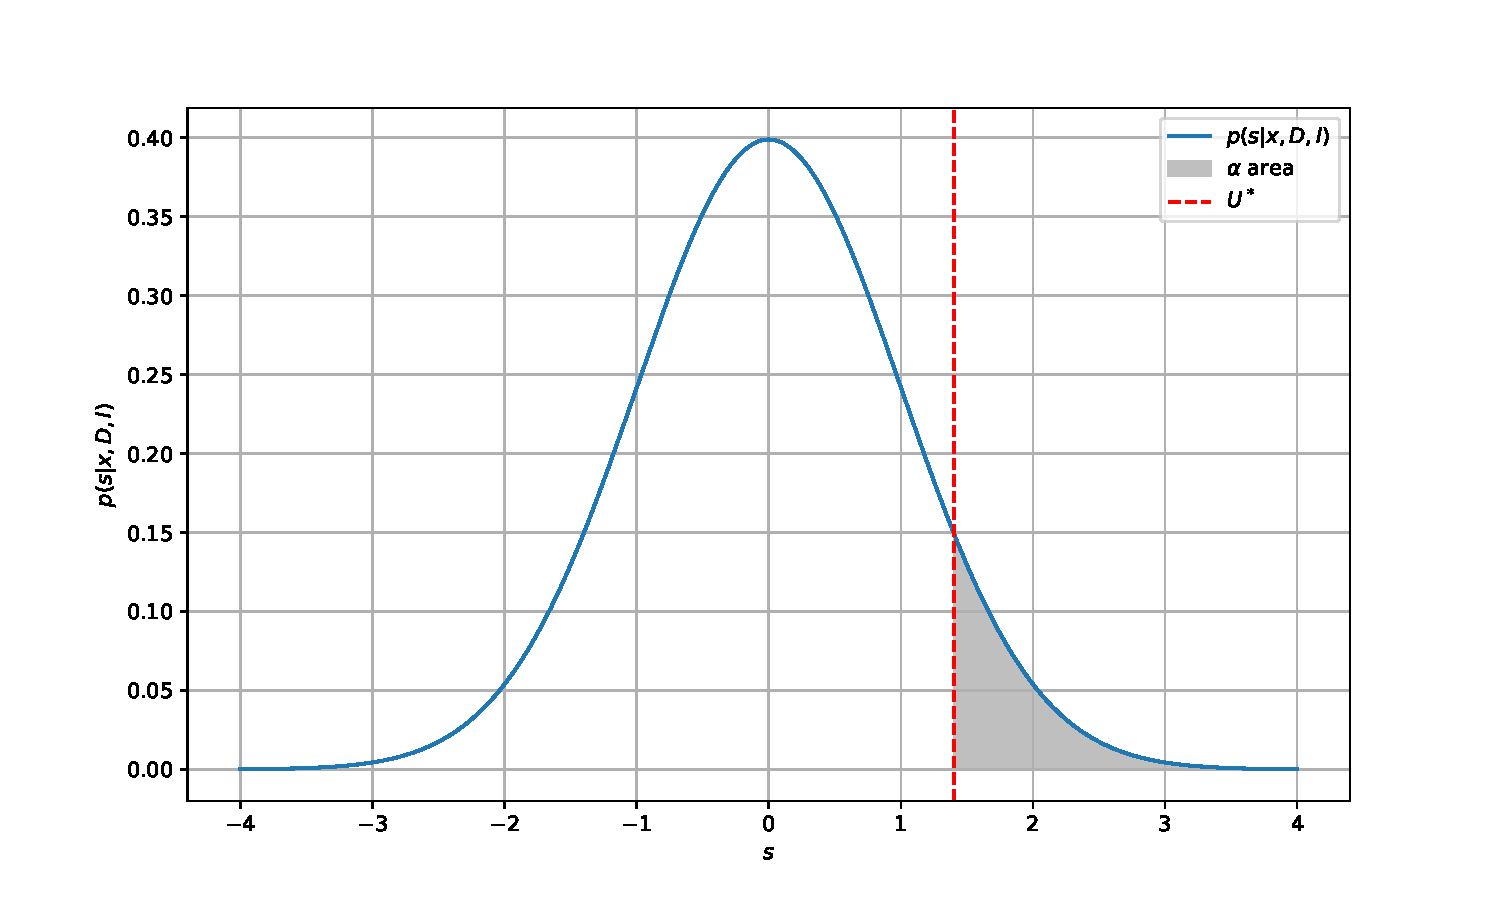
\includegraphics[width = 1\textwidth]{figures/alpha_plot.pdf}
		\caption{Illustration of equation \eqref{eq:decision} with $\alpha = 0.05$. A simple normal distribution has been used for illustrative purposes while it is understood equation \eqref{eq:decision} generalize beyond this simple setting.}
		\label{fig:2}
	\end{figure}
	\begin{figure}[H]
		\centering
		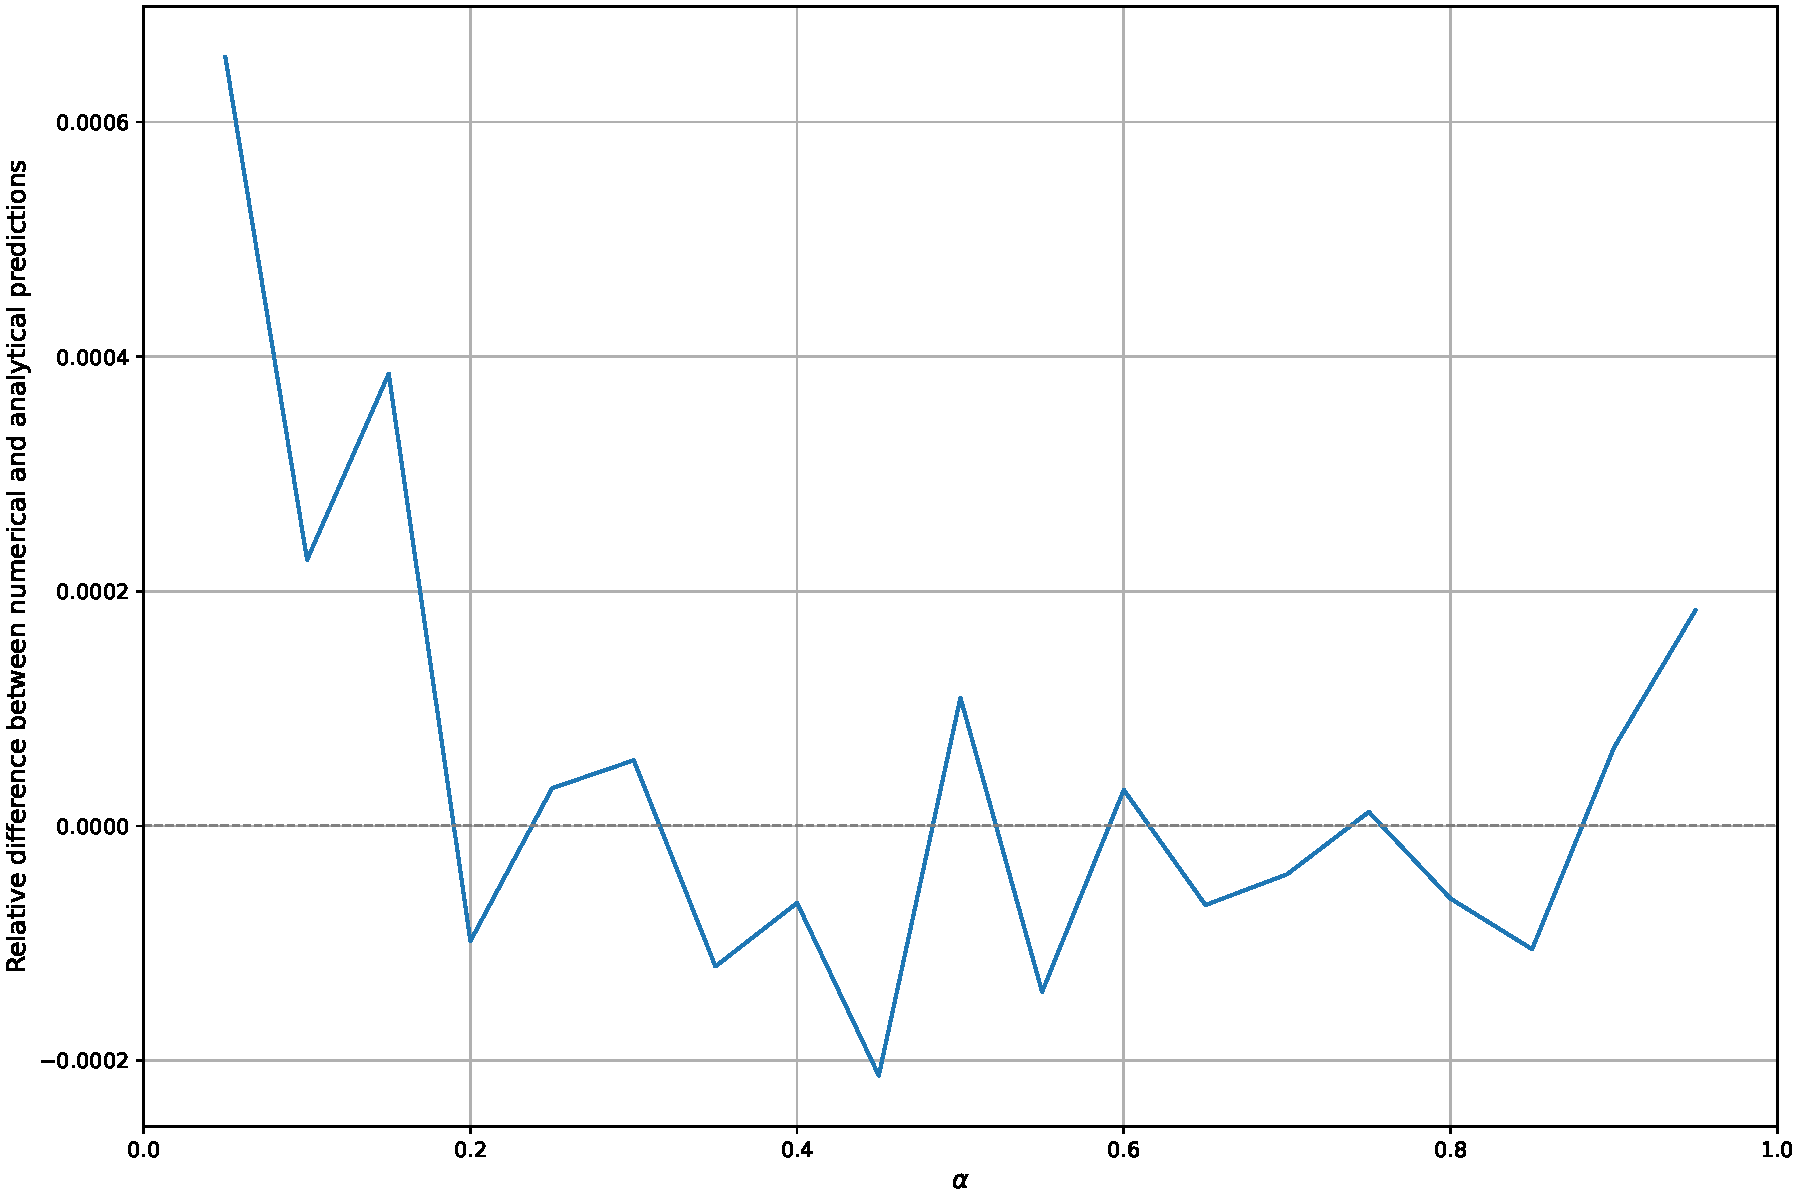
\includegraphics[width = 0.8\textwidth]{figures/numerical_example.pdf}
		\caption{The relative difference between numerically optimizing the expected cost and the percentile, as a function of $\alpha$.}
		\label{fig:3}
	\end{figure}
	
	\section{Summary and Discussion}	
	It has been shown how quantile regression can, using Bayesian decision theory, be derived as the optimal decision rule in case of an asymmetric linear cost function. Conversely, it can be deduced that any deviation from such a cost function will yield a different optimal decision rule.
	
	
	\bibliographystyle{plainnat}
	\bibliography{ref}
	
\end{document}